\documentclass{article}
\usepackage{amsmath,amssymb}
\usepackage{hyperref}
\usepackage{bm}

\newcommand{\yti}{Y_{Ti}}
\newcommand{\yci}{Y_{Ci}}
\newcommand{\uti}{U_{Ti}}
\newcommand{\uci}{U_{Ci}}
\newcommand{\etat}{\eta_T}
\newcommand{\etati}{\eta_{Ti}}

\newcommand{\mti}{\bar{m}_{Ti}}
\newcommand{\byt}{\bm{Y_T}}
\newcommand{\byc}{\bm{Y_C}}
\newcommand{\bmt}{\bm{\bar{m}_T}}
\newcommand{\bmi}{\bm{m}_i}
\newcommand{\bsi}{\bm{s}_i}

\newcommand{\EE}{\mathbb{E}}

\title{Data Analysis for 'The Role of Mastery Learning'}




\begin{document}
This document includes code to produce all of the results and run all
of the models reported in ``The Role of Mastery Learning in
Intelligent Tutoring Systems: Principal Stratification on a Latent Variable.''

The auxilliary files sourced here are available at our github repository,
\url{https://github.com/adamSales/ctaiAdvance}.

First, load in and transform the (pre-imputed) data:
\begin{kframe}
\begin{alltt}
\hlkwd{load}\hlstd{(}\hlstr{'data/HSdata.RData'}\hlstd{)}
\hlkwd{load}\hlstd{(}\hlstr{'data/advanceData.RData'}\hlstd{)}
\end{alltt}
\end{kframe}
We'll use the \texttt{R} package \texttt{rstan} to run the models:
\begin{kframe}
\begin{alltt}
\hlkwd{library}\hlstd{(rstan)}
\hlkwd{rstan_options}\hlstd{(}\hlkwc{auto_write} \hlstd{=} \hlnum{TRUE}\hlstd{)}
\hlkwd{options}\hlstd{(}\hlkwc{mc.cores} \hlstd{= parallel}\hlopt{::}\hlkwd{detectCores}\hlstd{())}
\end{alltt}
\end{kframe}

\section{Data Description (Section \ref{sec:data})}

This code produces the missigness information from Table 1, summarizing the student level data:
\begin{kframe}
\begin{alltt}
\hlstd{miss} \hlkwb{<-} \hlkwa{NULL}
\hlkwa{for}\hlstd{(i} \hlkwa{in} \hlkwd{c}\hlstd{(}\hlstr{'race'}\hlstd{,}\hlstr{'sex'}\hlstd{,}\hlstr{'spec'}\hlstd{,}\hlstr{'xirt'}\hlstd{)) miss} \hlkwb{<-} \hlkwd{rbind}\hlstd{(miss,}
 \hlkwd{c}\hlstd{(}\hlkwd{sum}\hlstd{(}\hlkwd{is.na}\hlstd{(covs[[i]])),}\hlkwd{mean}\hlstd{(}\hlkwd{is.na}\hlstd{(covs[[i]])),error[i,}\hlstr{'error'}\hlstd{]))}
\hlstd{miss} \hlkwb{<-} \hlkwd{as.data.frame}\hlstd{(miss)}
\hlstd{miss}\hlopt{$}\hlstd{`Error Type`} \hlkwb{<-} \hlkwd{c}\hlstd{(}\hlstr{'PFC'}\hlstd{,}\hlstr{'PFC'}\hlstd{,}\hlstr{'PFC'}\hlstd{,}\hlstr{'SRMSE'}\hlstd{)}
\hlkwd{rownames}\hlstd{(miss)} \hlkwb{<-} \hlkwd{c}\hlstd{(}\hlstr{'Race/Ethnicity'}\hlstd{,}\hlstr{'Sex'}\hlstd{,}\hlstr{'Special Education'}\hlstd{,}\hlstr{'Pretest'}\hlstd{)}
\hlkwd{names}\hlstd{(miss)[}\hlnum{1}\hlopt{:}\hlnum{3}\hlstd{]} \hlkwb{<-} \hlkwd{c}\hlstd{(}\hlstr{'# Missing'}\hlstd{,}\hlstr{'% Missing'}\hlstd{,}\hlstr{'Imputation Error'}\hlstd{)}
\hlstd{miss[,}\hlnum{2}\hlstd{]} \hlkwb{<-} \hlkwd{as.integer}\hlstd{(}\hlkwd{round}\hlstd{(miss[,}\hlnum{2}\hlstd{]}\hlopt{*}\hlnum{100}\hlstd{))}
\hlstd{miss[,}\hlnum{1}\hlstd{]} \hlkwb{<-} \hlkwd{as.integer}\hlstd{(miss[,}\hlnum{1}\hlstd{])}
\hlstd{miss[}\hlstr{'Pretest'}\hlstd{,}\hlstr{'Imputation Error'}\hlstd{]} \hlkwb{<-} \hlkwd{sqrt}\hlstd{(miss[}\hlstr{'Pretest'}\hlstd{,}\hlstr{'Imputation Error'}\hlstd{])}\hlopt{/}\hlkwd{sd}\hlstd{(covs}\hlopt{$}\hlstd{xirt,}\hlkwc{na.rm}\hlstd{=}\hlnum{TRUE}\hlstd{)}


\hlkwd{print}\hlstd{(xtable}\hlopt{::}\hlkwd{xtable}\hlstd{(miss))}
\end{alltt}
\end{kframe}% latex table generated in R 3.4.2 by xtable 1.8-2 package
% Tue Feb 06 15:01:52 2018
\begin{table}[ht]
\centering
\begin{tabular}{rrrrl}
  \hline
 & \# Missing & \% Missing & Imputation Error & Error Type \\ 
  \hline
Race/Ethnicity & 1071 &   8 & 0.23 & PFC \\ 
  Sex & 526 &   4 & 0.35 & PFC \\ 
  Special Education & 199 &   1 & 0.11 & PFC \\ 
  Pretest & 2367 &  18 & 0.20 & SRMSE \\ 
   \hline
\end{tabular}
\end{table}

This code produces the covariate balance information:
\begin{kframe}
\begin{alltt}
\hlstd{covBal} \hlkwb{<-} \hlkwa{NULL}
\hlkwa{for}\hlstd{(i} \hlkwa{in} \hlkwd{c}\hlstd{(}\hlstr{'race'}\hlstd{,}\hlstr{'sex'}\hlstd{,}\hlstr{'spec'}\hlstd{))\{}
    \hlstd{covBal} \hlkwb{<-} \hlkwd{rbind}\hlstd{(covBal,}\hlkwd{c}\hlstd{(i,}\hlnum{NA}\hlstd{,}\hlnum{NA}\hlstd{,}\hlnum{NA}\hlstd{,}\hlnum{NA}\hlstd{))}

    \hlkwa{for}\hlstd{(ll} \hlkwa{in} \hlkwd{levels}\hlstd{(dat[[i]]))\{}
        \hlstd{covBal} \hlkwb{<-} \hlkwd{rbind}\hlstd{(covBal,}\hlkwd{c}\hlstd{(}\hlnum{NA}\hlstd{,ll,}\hlkwd{round}\hlstd{(}\hlkwd{c}\hlstd{(}\hlkwd{mean}\hlstd{(dat[[i]]}\hlopt{==}\hlstd{ll),}\hlkwd{mean}\hlstd{(dat[[i]][dat}\hlopt{$}\hlstd{treatment}\hlopt{==}\hlnum{1}\hlstd{]}\hlopt{==}\hlstd{ll),}\hlkwd{mean}\hlstd{(dat[[i]][dat}\hlopt{$}\hlstd{treatment}\hlopt{==}\hlnum{0}\hlstd{]}\hlopt{==}\hlstd{ll)),}\hlnum{2}\hlstd{)))}

    \hlstd{\}}
\hlstd{\}}
\hlkwd{colnames}\hlstd{(covBal)} \hlkwb{<-} \hlkwd{c}\hlstd{(}\hlstr{'Covariate'}\hlstd{,}\hlstr{'Category'}\hlstd{,}\hlstr{'Overall Percent'}\hlstd{,}\hlstr{'Percent of Treated'}\hlstd{,}\hlstr{'Percent of Control'}\hlstd{)}
\hlkwd{print}\hlstd{(}\hlkwd{xtable}\hlstd{(covBal),}\hlkwc{floating}\hlstd{=}\hlnum{FALSE}\hlstd{,}\hlkwc{include.rownames}\hlstd{=}\hlnum{FALSE}\hlstd{)}
\end{alltt}
\end{kframe}% latex table generated in R 3.4.2 by xtable 1.8-2 package
% Tue Feb 06 15:46:52 2018
\begin{tabular}{lllll}
  \hline
Covariate & Category & Overall Percent & Percent of Treated & Percent of Control \\ 
  \hline
race &  &  &  &  \\ 
   & WhiteAsian & 0.49 & 0.52 & 0.47 \\ 
   & BlackMulti & 0.3 & 0.26 & 0.32 \\ 
   & HispAIAN & 0.21 & 0.22 & 0.21 \\ 
  sex &  &  &  &  \\ 
   & F & 0.5 & 0.49 & 0.51 \\ 
   & M & 0.5 & 0.51 & 0.49 \\ 
  spec &  &  &  &  \\ 
   & typical & 0.87 & 0.86 & 0.87 \\ 
   & speced & 0.08 & 0.08 & 0.08 \\ 
   & gifted & 0.05 & 0.06 & 0.05 \\ 
   \hline
\end{tabular}

The overall p-value for balance is:
\begin{knitrout}
\definecolor{shadecolor}{rgb}{0.969, 0.969, 0.969}\color{fgcolor}\begin{kframe}
\begin{alltt}
\hlkwd{library}\hlstd{(RItools)} \hlcom{## using development version}
\hlstd{balMod} \hlkwb{<-} \hlkwd{balanceTest}\hlstd{(treatment}\hlopt{~}\hlkwd{poly}\hlstd{(xirt,}\hlnum{2}\hlstd{)}\hlopt{+}\hlstd{spec}\hlopt{+}\hlstd{race}\hlopt{+}\hlstd{sex}\hlopt{+}\hlkwd{strata}\hlstd{(pair)}\hlopt{+}\hlkwd{cluster}\hlstd{(schoolid2),}\hlkwc{data}\hlstd{=datOrig,}\hlkwc{report}\hlstd{=}\hlstr{'chisquare.test'}\hlstd{)}
\hlkwd{print}\hlstd{(balMod}\hlopt{$}\hlstd{overall[}\hlstr{'pair'}\hlstd{,])}
\end{alltt}
\begin{verbatim}
## chisquare        df   p.value 
##    8.4464    7.0000    0.2949
\end{verbatim}
\end{kframe}
\end{knitrout}

\section{PS Model with $\bar{m}_T$}

Here we estimate the model in Section
\ref{sec:principalStratification} stratifying on $\bar{m}_T$.

First, we create the datasets:
\begin{kframe}
\begin{alltt}
\hlkwd{source}\hlstd{(}\hlstr{'R/prelimMbar.r'}\hlstd{)}
\end{alltt}
\end{kframe}

The model is encoded in the file \texttt{psmodObs.stan}.
It may be summarized as follows.
The model for $\bar{m}_T$ is:
\begin{equation}\label{eq:mbarUsage}
\bar{m}_{Ti}=\alpha^U_s+\bm{x}_i^T\bm{\beta^U}+\epsilon^{Ui}_i+\epsilon^{Ut}_{t[i]}
\end{equation}
where $\alpha^U_s$ is a separate intercept for each state, and $\bm{x}_i$ is a vector of covariates: dummy variables for
racial/ethnic category, a dummy variable for sex, dummy variables for
special education category, and linear and quadratic terms for
pretest.
The normally-distributed errors $\epsilon^{Ui}$ and $\epsilon^{Ut}_{t[i]}$ vary at the
individual and teacher levels.

The model for $Y$ is
\begin{equation}
Y_i=\alpha^Y_p+\bm{x}_i^T\bm{\beta^Y}+a_1\bar{m}_{Ti}+Z_i(b_0+b_1*\bar{m}_{Ti})+\epsilon^{Yi}_i+\epsilon^{Yt}_{t[i]}+\epsilon^{Ys}_{s[i]}
\end{equation}
where $\alpha^Y_p$ is a separate intercept for each randomization
block $p$, $Z_i$ is a dummy variable for treatment status,
$\epsilon^{Ys}_{s[i]}$ is a normally distributed error at the school
level, and the rest of the variables are analogous to those in
(\ref{eq:mbarUsage}).
We run the model with the \texttt{stan} command from \texttt{rstan}:
\begin{kframe}
\begin{alltt}
\hlstd{mbarMod} \hlkwb{<-} \hlkwd{stan}\hlstd{(}\hlstr{'R/psmodObs.stan'}\hlstd{,}\hlkwc{data}\hlstd{=sdat,}\hlkwc{seed}\hlstd{=}\hlnum{613}\hlstd{)}
\end{alltt}
\end{kframe}

Figure \ref{fig:mbarModel} can be replicated with the following code:

\begin{kframe}
\begin{alltt}
\hlkwd{library}\hlstd{(tikzDevice)} \hlcom{## allows latex code in figure}
\hlkwd{options}\hlstd{(} \hlkwc{tikzLatexPackages} \hlstd{=} \hlkwd{c}\hlstd{(}
\hlkwd{getOption}\hlstd{(} \hlstr{"tikzLatexPackages"} \hlstd{),}
\hlstr{"\textbackslash{}\textbackslash{}usepackage\{amsmath,amsfonts\}"}
\hlstd{))}

\hlstd{draw} \hlkwb{<-} \hlnum{1000}

\hlstd{samps} \hlkwb{<-} \hlkwd{extract}\hlstd{(mbarMod)}
\hlstd{plotDatObs} \hlkwb{<-} \hlkwd{with}\hlstd{(sdatObs,}\hlkwd{data.frame}\hlstd{(}\hlkwc{Y}\hlstd{=}\hlkwd{c}\hlstd{(YtO,YtM,Yc),}\hlkwc{mbar}\hlstd{=}\hlkwd{c}\hlstd{(MbarTO,samps}\hlopt{$}\hlstd{MbarTM[draw,],samps}\hlopt{$}\hlstd{MbarC[draw,]),}\hlkwc{Z}\hlstd{=}\hlkwd{c}\hlstd{(}\hlkwd{rep}\hlstd{(}\hlnum{1}\hlstd{,nstudTO),}\hlkwd{rep}\hlstd{(}\hlnum{1}\hlstd{,nstudTM),}\hlkwd{rep}\hlstd{(}\hlnum{0}\hlstd{,nstudC))))}
\hlstd{plotDatObs}\hlopt{$}\hlstd{treat} \hlkwb{<-} \hlkwd{ifelse}\hlstd{(plotDatObs}\hlopt{$}\hlstd{Z}\hlopt{==}\hlnum{1}\hlstd{,}\hlstr{'Treatment'}\hlstd{,}\hlstr{'Control'}\hlstd{)}
\hlstd{plotDatObs}\hlopt{$}\hlstd{slope} \hlkwb{<-} \hlkwd{ifelse}\hlstd{(plotDatObs}\hlopt{$}\hlstd{treat}\hlopt{==}\hlstr{'Control'}\hlstd{,samps}\hlopt{$}\hlstd{a1[draw],samps}\hlopt{$}\hlstd{a1[draw]}\hlopt{+}\hlstd{samps}\hlopt{$}\hlstd{b1[draw])}
\hlstd{plotDatObs}\hlopt{$}\hlstd{int} \hlkwb{<-} \hlkwd{ifelse}\hlstd{(plotDatObs}\hlopt{$}\hlstd{treat}\hlopt{==}\hlstr{'Control'}\hlstd{,samps}\hlopt{$}\hlstd{a0[draw],samps}\hlopt{$}\hlstd{a0[draw]}\hlopt{+}\hlstd{samps}\hlopt{$}\hlstd{b0[draw])}

\hlstd{plotDatObs} \hlkwb{<-} \hlkwd{within}\hlstd{(plotDatObs, int} \hlkwb{<-} \hlstd{int}\hlopt{-}\hlstd{(} \hlkwd{mean}\hlstd{(int}\hlopt{+}\hlstd{slope}\hlopt{*}\hlstd{mbar)}\hlopt{-}\hlkwd{mean}\hlstd{(plotDatObs}\hlopt{$}\hlstd{Y)))}
\hlstd{plotDatObs} \hlkwb{<-} \hlstd{plotDatObs[}\hlkwd{order}\hlstd{(plotDatObs}\hlopt{$}\hlstd{treat),]}
\hlstd{plotDatObs}\hlopt{$}\hlstd{treat2} \hlkwb{<-} \hlstd{plotDatObs}\hlopt{$}\hlstd{treat}

\hlkwd{tikz}\hlstd{(}\hlkwc{file} \hlstd{=} \hlstr{"figure/mbarModel.tex"}\hlstd{,}
  \hlkwc{standAlone} \hlstd{= T,}
  \hlkwc{width}  \hlstd{=} \hlnum{6}\hlstd{,} \hlkwc{height}  \hlstd{=} \hlnum{3}\hlstd{)}

\hlkwd{ggplot}\hlstd{(plotDatObs,}\hlkwd{aes}\hlstd{(mbar,Y,}\hlkwc{fill}\hlstd{=treat,}\hlkwc{group}\hlstd{=treat,}\hlkwc{alpha}\hlstd{=treat,}\hlkwc{color}\hlstd{=treat))}\hlopt{+}\hlkwd{geom_point}\hlstd{(}\hlkwc{size}\hlstd{=}\hlnum{2}\hlstd{)}\hlopt{+}
    \hlkwd{geom_abline}\hlstd{(}\hlkwd{aes}\hlstd{(}\hlkwc{intercept}\hlstd{=int,}\hlkwc{slope}\hlstd{=slope,}\hlkwc{linetype}\hlstd{=treat2),}\hlkwc{color}\hlstd{=}\hlstr{'black'}\hlstd{,}\hlkwc{size}\hlstd{=}\hlnum{2}\hlstd{,}\hlkwc{alpha}\hlstd{=}\hlnum{1}\hlstd{)}\hlopt{+}\hlkwd{scale_alpha_discrete}\hlstd{(}\hlkwc{range}\hlstd{=}\hlkwd{c}\hlstd{(}\hlnum{0.4}\hlstd{,}\hlnum{.8}\hlstd{))}\hlopt{+}
    \hlkwd{scale_colour_manual}\hlstd{(}\hlkwc{values}\hlstd{=}\hlkwd{c}\hlstd{(}\hlstr{'red'}\hlstd{,}\hlstr{'blue'}\hlstd{))}\hlopt{+}
    \hlkwd{labs}\hlstd{(}\hlkwc{group}\hlstd{=}\hlkwa{NULL}\hlstd{,}\hlkwc{fill}\hlstd{=}\hlkwa{NULL}\hlstd{,}\hlkwc{alpha}\hlstd{=}\hlkwa{NULL}\hlstd{)}\hlopt{+}\hlkwd{xlab}\hlstd{(}\hlstr{'$\textbackslash{}\textbackslash{}bar\{m\}_T$'}\hlstd{)}\hlopt{+}
    \hlkwd{ylab}\hlstd{(}\hlstr{'Posttest Score'}\hlstd{)}\hlopt{+}\hlkwd{theme}\hlstd{(}\hlkwc{legend.position}\hlstd{=}\hlstr{'top'}\hlstd{,}\hlkwc{text}\hlstd{=}\hlkwd{element_text}\hlstd{(}\hlkwc{size}\hlstd{=}\hlnum{20}\hlstd{))}\hlopt{+}
    \hlkwd{guides}\hlstd{(}\hlkwc{color} \hlstd{=} \hlkwd{guide_legend}\hlstd{(}\hlkwc{title}\hlstd{=}\hlkwa{NULL}\hlstd{,}\hlkwc{override.aes}\hlstd{=}\hlkwd{list}\hlstd{(}\hlkwc{alpha}\hlstd{=}\hlnum{1}\hlstd{),}\hlkwc{keywidth}\hlstd{=}\hlnum{3}\hlstd{),}\hlkwc{linetype}\hlstd{=}\hlkwd{guide_legend}\hlstd{(}\hlkwc{title}\hlstd{=}\hlkwa{NULL}\hlstd{,}\hlkwc{keywidth}\hlstd{=}\hlnum{1}\hlstd{))}\hlcom{#override.aes=list(size=2)))}
\hlkwd{dev.off}\hlstd{()}
\end{alltt}
\end{kframe}pdf 
  2 
\begin{kframe}\begin{alltt}
\hlkwd{setwd}\hlstd{(}\hlstr{'figure'}\hlstd{); tools}\hlopt{::}\hlkwd{texi2dvi}\hlstd{(}\hlstr{'mbarModel.tex'}\hlstd{,} \hlkwc{pdf} \hlstd{= T,} \hlkwc{clean} \hlstd{= T);} \hlkwd{setwd}\hlstd{(}\hlstr{'..'}\hlstd{)}
\end{alltt}
\end{kframe}
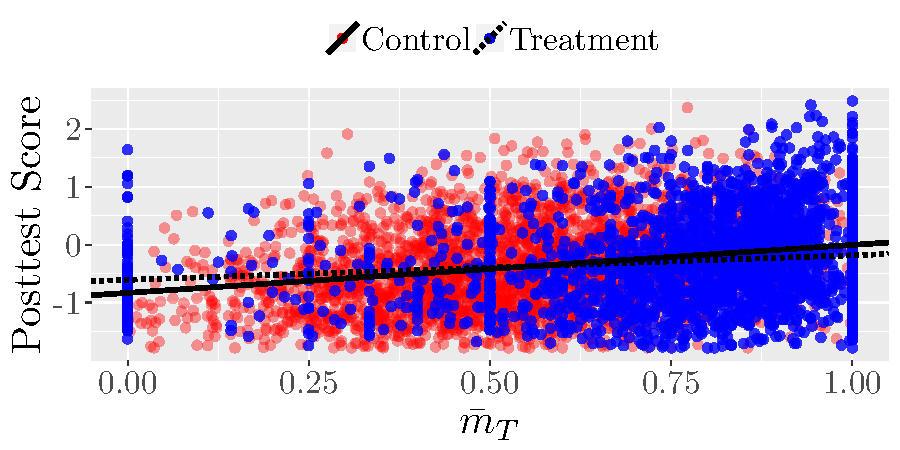
\includegraphics{figure/mbarModel.pdf}

To save memory, save and delete the $\bar{m}_T$ model:
\begin{kframe}
\begin{alltt}
\hlkwd{save}\hlstd{(mbarMod,}\hlkwc{file}\hlstd{=}\hlstr{'fittedModels/mbarMod.RData'}\hlstd{)}
\end{alltt}
\end{kframe}
\begin{knitrout}
\definecolor{shadecolor}{rgb}{0.969, 0.969, 0.969}\color{fgcolor}\begin{kframe}
\begin{alltt}
\hlkwd{rm}\hlstd{(mbarMod);} \hlkwd{gc}\hlstd{()}
\end{alltt}
\end{kframe}
\end{knitrout}


\section{The Main PS Model}
This section reproduces our paper's main model, described in Section \ref{sec:themodel}.

The data for the main model (similar to the $\bar{m}$ model but
including student-section level mastery data) relies on a secondary
file (available at github):
\begin{kframe}
\begin{alltt}
\hlkwd{source}\hlstd{(}\hlstr{'R/prelimStan.r'}\hlstd{)}
\end{alltt}
\end{kframe}

\newpage
Since this is the main model, we will include full stan code in this
online supplement:
\begin{verbatim}
data{
//Sample sizes
 int<lower=1> nsecWorked;
 int<lower=1> ncov;
 int<lower=1> nstud;
 int<lower=1> nteacher;
 int<lower=1> nsec;
 int<lower=1> nschool;
 int<lower=1> npair;

// indices
 int<lower=1,upper=nteacher> teacher[nstud];
 int<lower=1,upper=npair> pair[nstud];
 int<lower=1,upper=nschool> school[nstud];
 int<lower=1,upper=nstud> studentM[nsecWorked];
 int<lower=1,upper=nsec> section[nsecWorked];

// data data
 int<lower=0,upper=1> grad[nsecWorked];
 matrix[nstud,ncov] X;
 int<lower=0,upper=1> Z[nstud];
 real Y[nstud];

}
parameters{

 vector[nstud] studEff;

 vector[ncov] betaU;
 vector[ncov] betaY;

 real a0;
 real a1;
 real b0;
 real b1;

 real teacherEffY[nteacher];
 real teacherEffU[nteacher];
 real pairEffect[npair];
 real schoolEffU[nschool];
 real schoolEffY[nschool];
 real secEff[nsec];

 real<lower=0> sigTchY;
 real<lower=0> sigSclY;
 real<lower=0> sigY[2];
 real<lower=0> sigTchU;
 real<lower=0> sigSclU;
 real<lower=0> sigU;
}

model{
 real linPred[nsecWorked];
 vector[nstud] muY;
 vector[nstud] muU;
 real useEff[nstud];
 real trtEff[nstud];
 real sigYI[nstud];


// grad model
 for(i in 1:nsecWorked)
  linPred[i]= secEff[section[i]]+studEff[studentM[i]];

 for(i in 1:nstud){
  useEff[i]=a0+a1*studEff[i];
  trtEff[i]=b0+b1*studEff[i];
  muU[i]=teacherEffU[teacher[i]]+schoolEffU[school[i]];
  muY[i]=teacherEffY[teacher[i]]+schoolEffY[school[i]]+pairEffect[pair[i]]+useEff[i]+Z[i]*trtEff[i];
  sigYI[i]=sigY[Z[i]+1];
 }

 //priors
 betaY~normal(0,2);
 betaU~normal(0,2);
 pairEffect~normal(0,2);

 a0~normal(0,1);
 a1~normal(0,1);
 b0~normal(0,1);
 b1~normal(0,1);


 schoolEffY~normal(0,sigSclY);
 schoolEffU~normal(0,sigSclU);
 teacherEffU~normal(0,sigTchU);
 teacherEffY~normal(0,sigTchY);

 grad~bernoulli_logit(linPred);

 studEff~normal(muU+X*betaU,sigU);
 Y~normal(muY+X*betaY,sigYI);
}

\end{verbatim}

This code runs the model:
\begin{kframe}
\begin{alltt}
\hlstd{main} \hlkwb{<-} \hlkwd{stan}\hlstd{(}\hlstr{'src/psmod.stan'}\hlstd{,}\hlkwc{data} \hlstd{=sdat,}\hlkwc{warmup}\hlstd{=}\hlnum{1500}\hlstd{,}\hlkwc{chains}\hlstd{=}\hlnum{10}\hlstd{,}\hlkwc{iter}\hlstd{=}\hlnum{5000}\hlstd{)}
\end{alltt}
\end{kframe}

\section{Multiple Imputation Model Fit}

To give some intuition on how the model fitting worked, and to what
extent treatment effect moderation was discernable in this dataset
anyway, we re-fit the model using (something akin to) multiple
imputation.
First, extract 1000 random draws of $\eta_T$ (denoted as
\texttt{studEff} in the model code) from the fitted model.
Then, for each draw, fit a standard HLM interacting treatment with the
$\eta_T$ draw.










